\chapter{Παραρτήματα}
		
\section{Διάρθρωση Ομάδας και Κατανομή Αρμοδιοτήτων}

\noindent
\textbf{Ιωάννης Χαλκιόπουλος}
\begin{enumerate}
	\item 2.3 - Αρχιτεκτονική και Πλατφόρμα Τρέχοντος Συστήματος  (Εξ’ ολοκλήρου)
	\item 3.2 - Μή Λειτουργικές Απαιτήσεις  (Εξ’ ολοκλήρου)
	\item Συμμετοχή στις συναντήσεις με τον υπεύθυνο της επιχείρησης
\end{enumerate}

\noindent
\textbf{Αντώνης Χαλκιάς}
\begin{enumerate}
\item 2.2 - Περιγραφή Τρέχοντος Συστήματος Πελάτη (Εξ’ ολοκλήρου)
\item 4.2 - Εμπορικά Πακέτα Λογισμικού: Παρουσίαση suitepad (σε συνεργασία με Αλέξανδρο Τογρίδη) και Οικονομική ανάλυση για Suitepad και 
			Mini Hotel (Εξ’ ολοκλήρου)
\item 4.3 - Επιλογή Ανάπτυξης Νέου Συστήματος: Οικονομική ανάλυση και να ανάλυση χρονοδιαγράμματος (Εξ’ ολοκλήρου)
\item 5.3 - Διαγράμματα Ακολουθίας (Sequence diagram) επιπέδου σχεδίασης (Εξ’ ολοκλήρου)
\item Συμμετοχή στις συναντήσεις με τον υπεύθυνο της επιχείρησης
\end{enumerate}

\noindent
\textbf{Άγγελος Κοντογιάννης}
\begin{enumerate}
	\item 2.1 - οργανωτικό διάγραμμα (Εξ’ ολοκλήρου)
	\item 4.2 - Εμπορικά Πακέτα Λογισμικού (σε συνεργασία με Αντώνη Χαλκιά)
	\item 4.3 - Επιλογή Ανάπτυξης Νέου Συστήματος (σε συνεργασία με Αντώνη Χαλκιά)
	\item 4.4 - Τελική Πρόταση (Εξ’ ολοκλήρου)
	\item 5.5 - State Machine Diagrams (Εξ’ ολοκλήρου)
	\item 6.3 - Πηγές
	\item 6.4 - Πρακτικά Συναντήσεων
	\item Συμμετοχή στις συναντήσεις με τον υπεύθυνο της επιχείρησης
\end{enumerate}

\noindent
\\\textbf{Αλέξανδρος Τογρίδης}
\begin{enumerate}
	\item Εxecutive Summary (Εξ’ ολοκλήρου)
	\item 1 - Εισαγωγή (Εξ’ ολοκλήρου)
	\item 2.4 – Πλεονεκτήματα, Αδυναμίες, Ευκαιρίες και Απειλές (Εξ’ ολοκλήρου)
	\item 4.1 – Κριτήρια Αξιολόγησης Επιλογών (Εξ’ ολοκλήρου)
	\item 4.2 – Εμπορικά πακέτα Λογισμικού  Ανάλυση του πακέτου Suitepad (σε συνεργασία με Αντώνης Χαλκιάς)
	\item 5.4 – Διαγράμματα Ακολουθίας (Sequence diagram) επιπέδου σχεδίασης (Εξ’ ολοκλήρου)
	\item Συντακτική και ορθογραφική επιμέλεια μέρους της τελικής εργασίας (Σε συνεργασία με Αλέξανδρο Σταυρόπουλο)
	\item Συμμετοχή στις συναντήσεις με τον υπεύθυνο της επιχείρησης
\end{enumerate}

\noindent
\\\textbf{Αλέξανδρος-Ανδρέας Σταυρόπουλος}
\begin{enumerate}
	\item 2.5 - Εμβέλεια Έργου και Περιορισμοί Κύκλου Έργου (Εξ'ολοκλήρου)
	\item 3.1 - Λειτουργικές Απαιτήσεις (Εξ'ολοκλήρου)
	\item 5.1 - Διαγράμματα Περιπτώσεων Χρήσης (use case diagrams) (Εξ'ολοκλήρου)
	\item 5.2 - Διαγράμματα Δραστηριοτήτων (Activity diagrams) (Εξ'ολοκλήρου)
	\item 6.1 - Διάρθρωση Ομάδας και Κατανομή Αρμοδιοτήτων (Εξ'ολοκλήρου)
	\item 6.2 - Ερωτηματολόγιο Εντοπισμού Απαιτήσεων Λειτουργίας Συστήματος (Εξ'ολοκλήρου)
	\item Επιμέλεια κώδικα latex (Εξ'ολοκλήρου)
	\item Συντακτική και ορθογραφική επιμέλεια μέρους της τελικής εργασίας (Σε συνεργασία με Αλέξανδρο Σταυρόπουλο)
	\item Συμμετοχή στις συναντήσεις με τον υπεύθυνο της επιχείρησης
\end{enumerate}


\section{Ερωτηματολόγιο Εντοπισμού Απαιτήσεων Λειτουργίας Συστήματος}
\textbf{1) Πείτε μας κάποιες βασικές πληροφορίες όπως έτος ίδρυσης, αριθμός 
	υπαλλήλων που απασχολούνται και συνεργαζόμενες εταιρείες.} \\
\noindent
Η επιχείρηση ξεκίνησε την λειτουργία της τον χειμώνα του 2020, απασχολεί κατά 
το μέγιστο 5 άτομα,(ποιοι είναι οι ρόλοι) και συνεργάζεται με μία επιχείρηση
για την προμήθεια καθαριστικών, 3 για τον ανεφοδιασμό τροφίμων, και μία για 
τα κλινοσκεπάσματα και τα λευκά είδη. \\

\noindent
\textbf{2) Πείτε μας με ποιούς τρόπους μπορεί ένας πελάτης να επικοινωνήσει
	με τον κατάλυμα ώστε να ενημερωθεί για τις παροχές του και να γίνει κράτηση
	σε αυτό.} \\
\noindent
Αυτή τη στιγμή το κατάλυμα δεν διαθέτει κάποιου είδους site αλλά ο πελάτης
μπορεί να το βρει μέσω πλατφορμών όπως 	E-Booking και Xpedia και να κάνει
κράτηση είτε μέσω site είτε μέσω τηλεφώνου. \\
  
\noindent
\textbf{3) Πείτε μας ποιός είναι ο μέγιστος αριθμός πελατών που μπορεί να φιλοξενήσει 
	το κατάλυμα και πόσα τα δωμάτια αυτά.} \\
\noindent
Το κατάλυμα διαθέτει 9 δωμάτια εκ των οποίων τα 8 είναι δίκλινα και το ένα τρίκλινο.
και ως αποτέλεσμα έχει τη δυνατότητα να φιλοξενεί έως και 19 άτομα.\\

\noindent
\textbf{4) Πότε παρουσιάζεται η μεγαλύτερη κινητικότητα στο ξενοδοχείο.} \\
\noindent
Μεγαλύτερη κινητικότητα παρατηρείται κατά τους καλοκαιρινούς μήνες όπου 
και ο αριθμός των τουριστών, είναι ο μεγαλύτερος.\\

\noindent
\textbf{5) Ποιές είναι οι απαραίτητες πληροφορίες για κάθε πελάτη.} \\
\noindent
Κατά κύριο λόγο, οι πληροφορίες που ζητούνται από τον πελάτη είναι 
το όνομα επίθετο και η ημερομηνία άφιξης. \\

\noindent
\textbf{6) Με ποιό τρόπο αποθηκεύονται αυτές οι πληροφορίες.} \\
\noindent
Οι πληροφορίες αυτές βρίσκονται σε ηλεκτρονική μορφή στον κεντρικό υπολογιστή
του καταλύματος ως backup αλλά και σε φυσική μορφή καθώς έτσι είναι το νόμιμο. \\

\noindent
\textbf{7) Με ποιούς τρόπους μπορεί ένας πελάτης μπορεί  να επικοινωνήσει 
	με τον υπεύθυνο ή να αιτηθεί κάποια από τις παρεχόμενες παροχές.} \\
\noindent
Ο πελάτης έχει τη δυνατότητα να επικοινωνήσει με την υποδοχή μέσω τηλεφώνου
είτε με φυσική παρουσία, εάν κατέβει στην υποδοχή.\\

\noindent
\textbf{8) Πείτε μας με ποιές παροχές παρέχονται στους πελάτες κατά την διαμονή 
	του στο κατάλυμα.} \\
\noindent
Στον πελάτη, στην παρούσα φάση, παρέχονται οι εξής παροχές: τζακούζι,  έξυπνες λάμπες
και smart tv, tablet, φαγητό στο δωμάτιο, πρωινό  καθώς και μία μικρή κάβα. Ακόμα,
παρέχονται πληροφορίες για τα Χανιά.\\

\noindent
\textbf{9) Πείτε μας με ποιούς τρόπους μπορεί το κατάλυμα να επικοινωνήσει με τις 
	συνεργαζόμενες εταιρείες.} \\
\noindent
Στην παρούσα φάση, το κατάλυμα επικοινωνεί με τις συνεργαζόμενες επιχειρήσεις
μέσω τηλεφώνου ή Email.\\

\noindent
\textbf{10) Πείτε μας κάποιες βασικές λειτουργίες που εκτελούνται με το υπάρχον 
	σύστημα.}\\
Στο παρόν σύστημα, εκτελούνται οι εξής λειτουργίες. Πρώτον ο πελάτης μπορεί να
παραγγείλει κάποιο γεύμα στο δωμάτιο και δεύτερον γίνεται η καταγραφή των 
απωλειών από κάθε δωμάτιο μετά το τέλος διαμονής ενός πελάτη.\\

\noindent
\textbf{11) Κατά την διάρκεια της πανδημίας, παρουσιάστηκαν διαφορές στην
	λειτουργία του καταλύματος.} \\
Κατά την διάρκεια της πανδημίας, έγινε υποχρεωτική και καταγραφή της χώρας
προέλευσης του πελάτη για τις περιπτώσεις όπου υπάρχει κρούσμα covid. \\ 

\noindent
\textbf{12) Τι λειτουργίες θα θέλατε να κάνει το σύστημα και με τι βαθμό 
	προτεραιότητας.} \\
Βασικές λειτουργίες του συστήματος θα είναι η λίστα με τις συχνές ερωτήσεις 
καθώς και η επικοινωνία μέσω chat με τον πελάτη, ενώ αν είναι εφικτό να υπάρχει
η λειτουργία μέσω της οποία θα μπορεί να κάνει παραγγελίες και τελευταία όσον 
αφορά τις προτεραιότητες, είναι η δυνατότητα καταγραφής και αναφοράς απωλειών
από τα δωμάτια. 

\clearpage
\section{Βιβλιογραφία και Πηγές Πληροφοριών}
\begin{itemize}
	\item Διαφάνειες Μαθήματος (Θεωρία - Φροντιστήρια)
	\item \href{ https://www.virtualemployee.com/lp/hire-software-developers-india-i/?source=google&medium=cpc&keyword=hire%20a%20software%20engineer&matchtype=b&device=c&campaign=software_development&adgroup=hire_software_engineer_tier1&pos=&net=g&gclid=CjwKCAiAz--OBhBIEiwAG1rIOkDiYrKWjAVtcSgXdPYeqNjCHwsJ2hvWdK-TsnGWImbc7NJc1j4eFBoCCLQQAvD_BwE }{Τιμή προγραμματιστικής ομάδας}
	\item \href{https://www.suitepad.de/de/ }{Suitepad}
	\item \href{https://hoteltechreport.com/guest-experience/guest-room-tablets/suitepad}{Κριτικές/πληροφορίες σχετικά με το Suitepad}
	\item \href{https://wiki.scn.sap.com/wiki/display/WHP/Workload+Analysis+and+Response+times}{Response times database server}
	\item \href{https://docs.microsoft.com/en-us/sharepoint/administration/storage-and-sql-server-capacity-planning-and-configuration}
				{Database file size}
	\item \href{https://dba.stackexchange.com/questions/185419/tde-encryption-on-database-tripled-size-of-backup-files}
				{Encrypted database file size 1}
	\item \href{https://security.stackexchange.com/questions/117068/why-would-an-encrypted-file-be-35-larger-than-an-unencrypted-one}
				{Encrypted database file size 2}	
	\item \href{https://db-engines.com/en/ranking/relational+dbms}{Types of SQL rankings}
\end{itemize}
\clearpage
\section{Πρακτικά Συναντήσεων}
\begin{figure}[H]
	\centering
	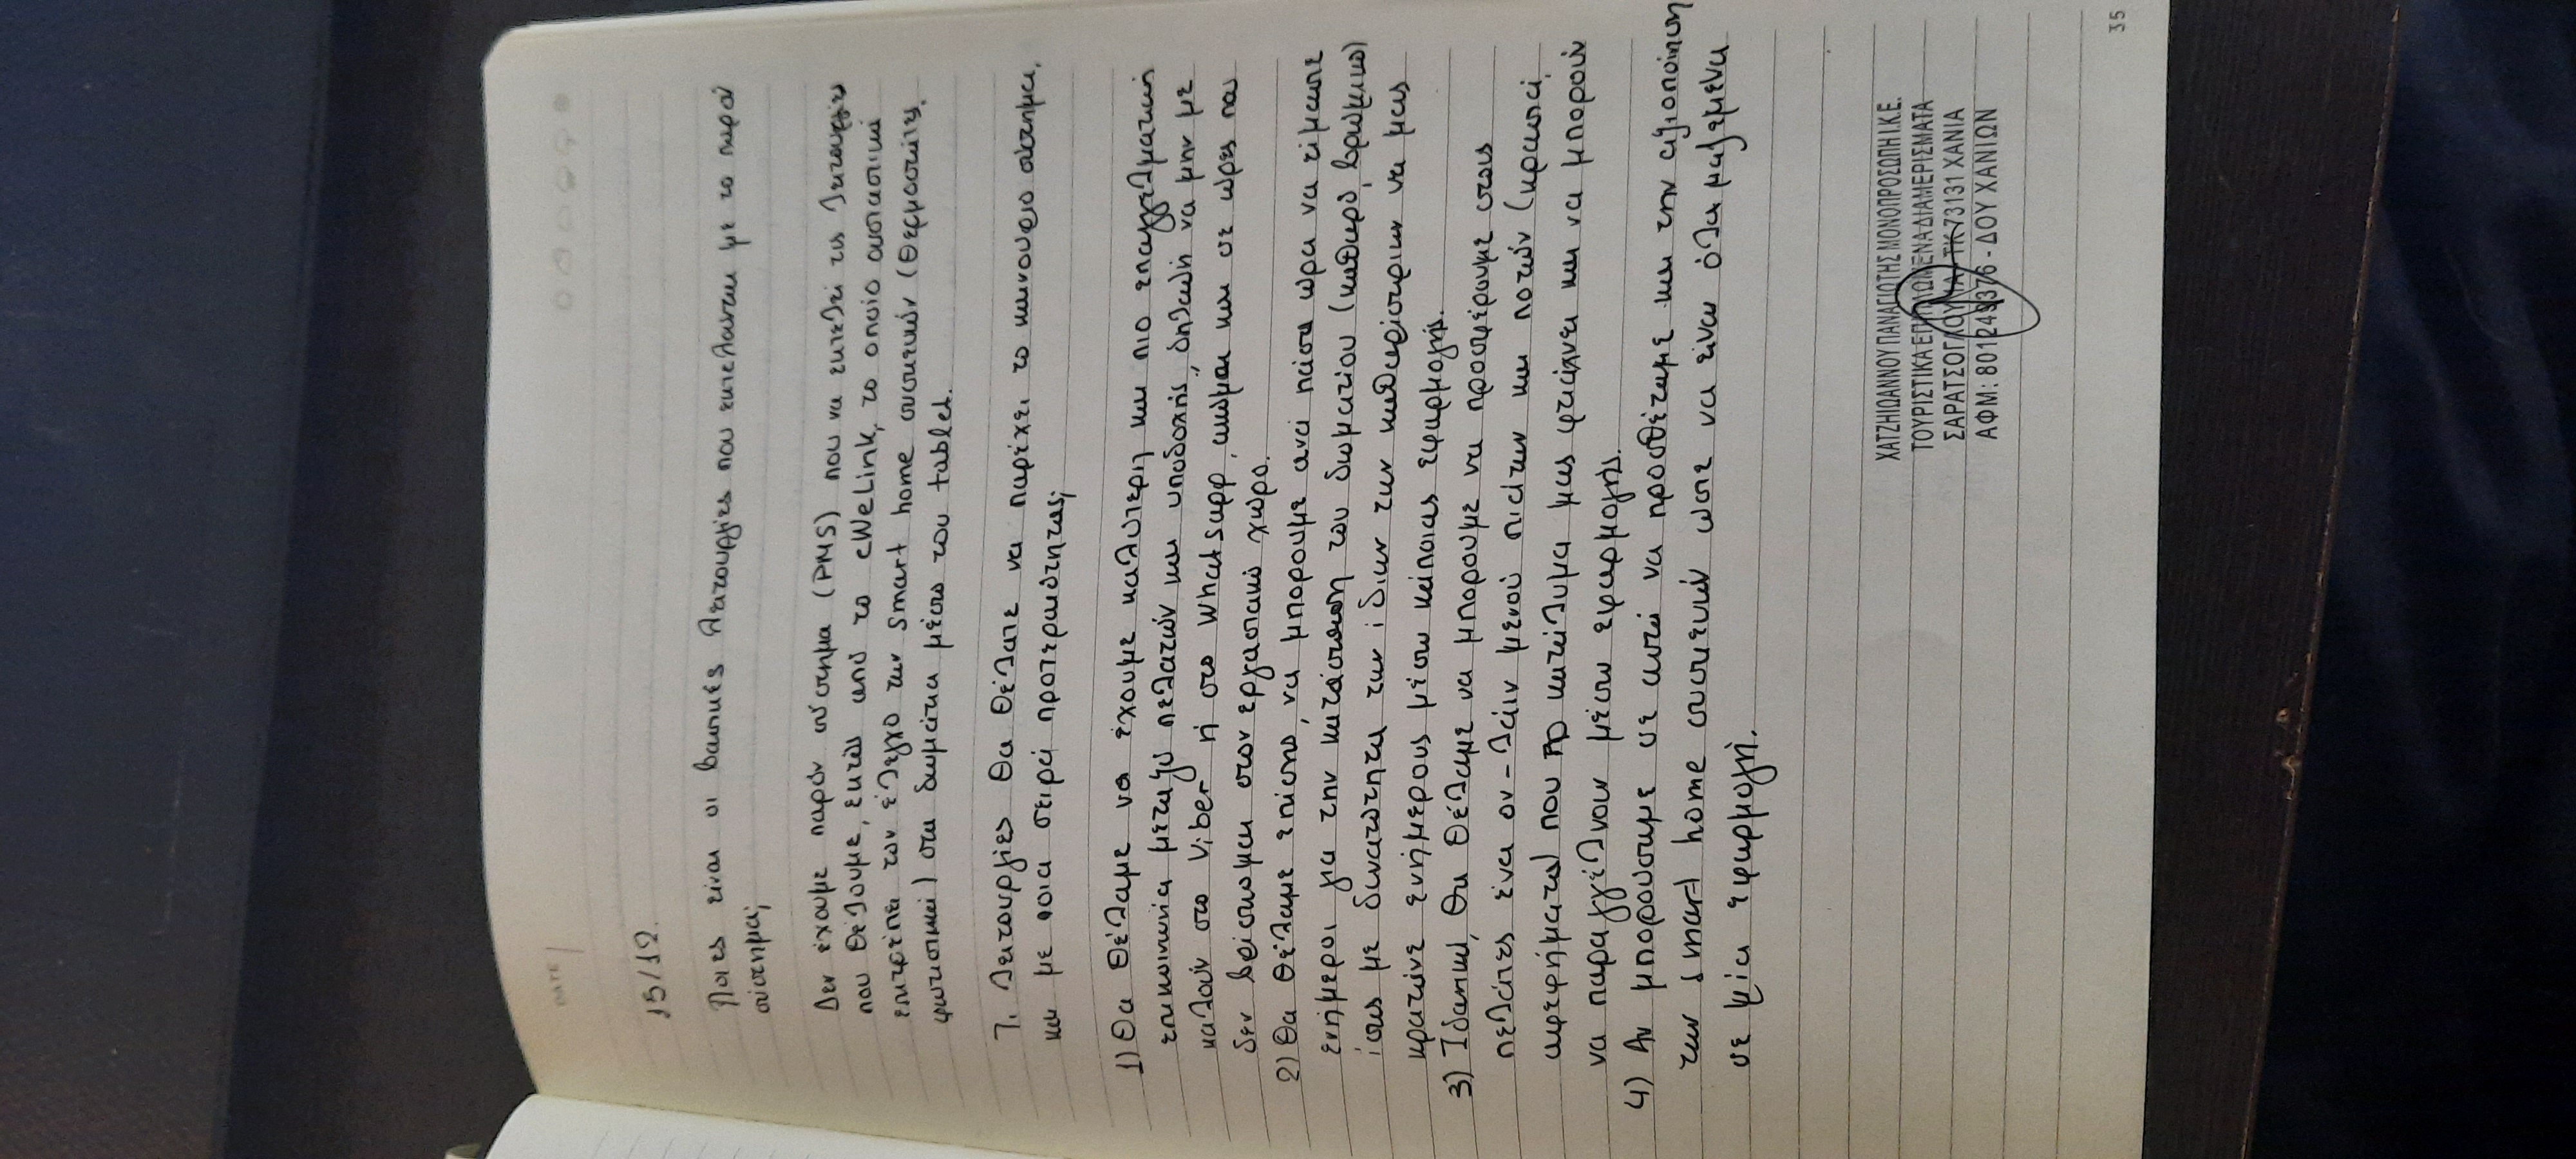
\includegraphics[angle=270, width=0.4\textwidth]{Images/p1}
\end{figure}

\begin{figure}[H]
	\centering
	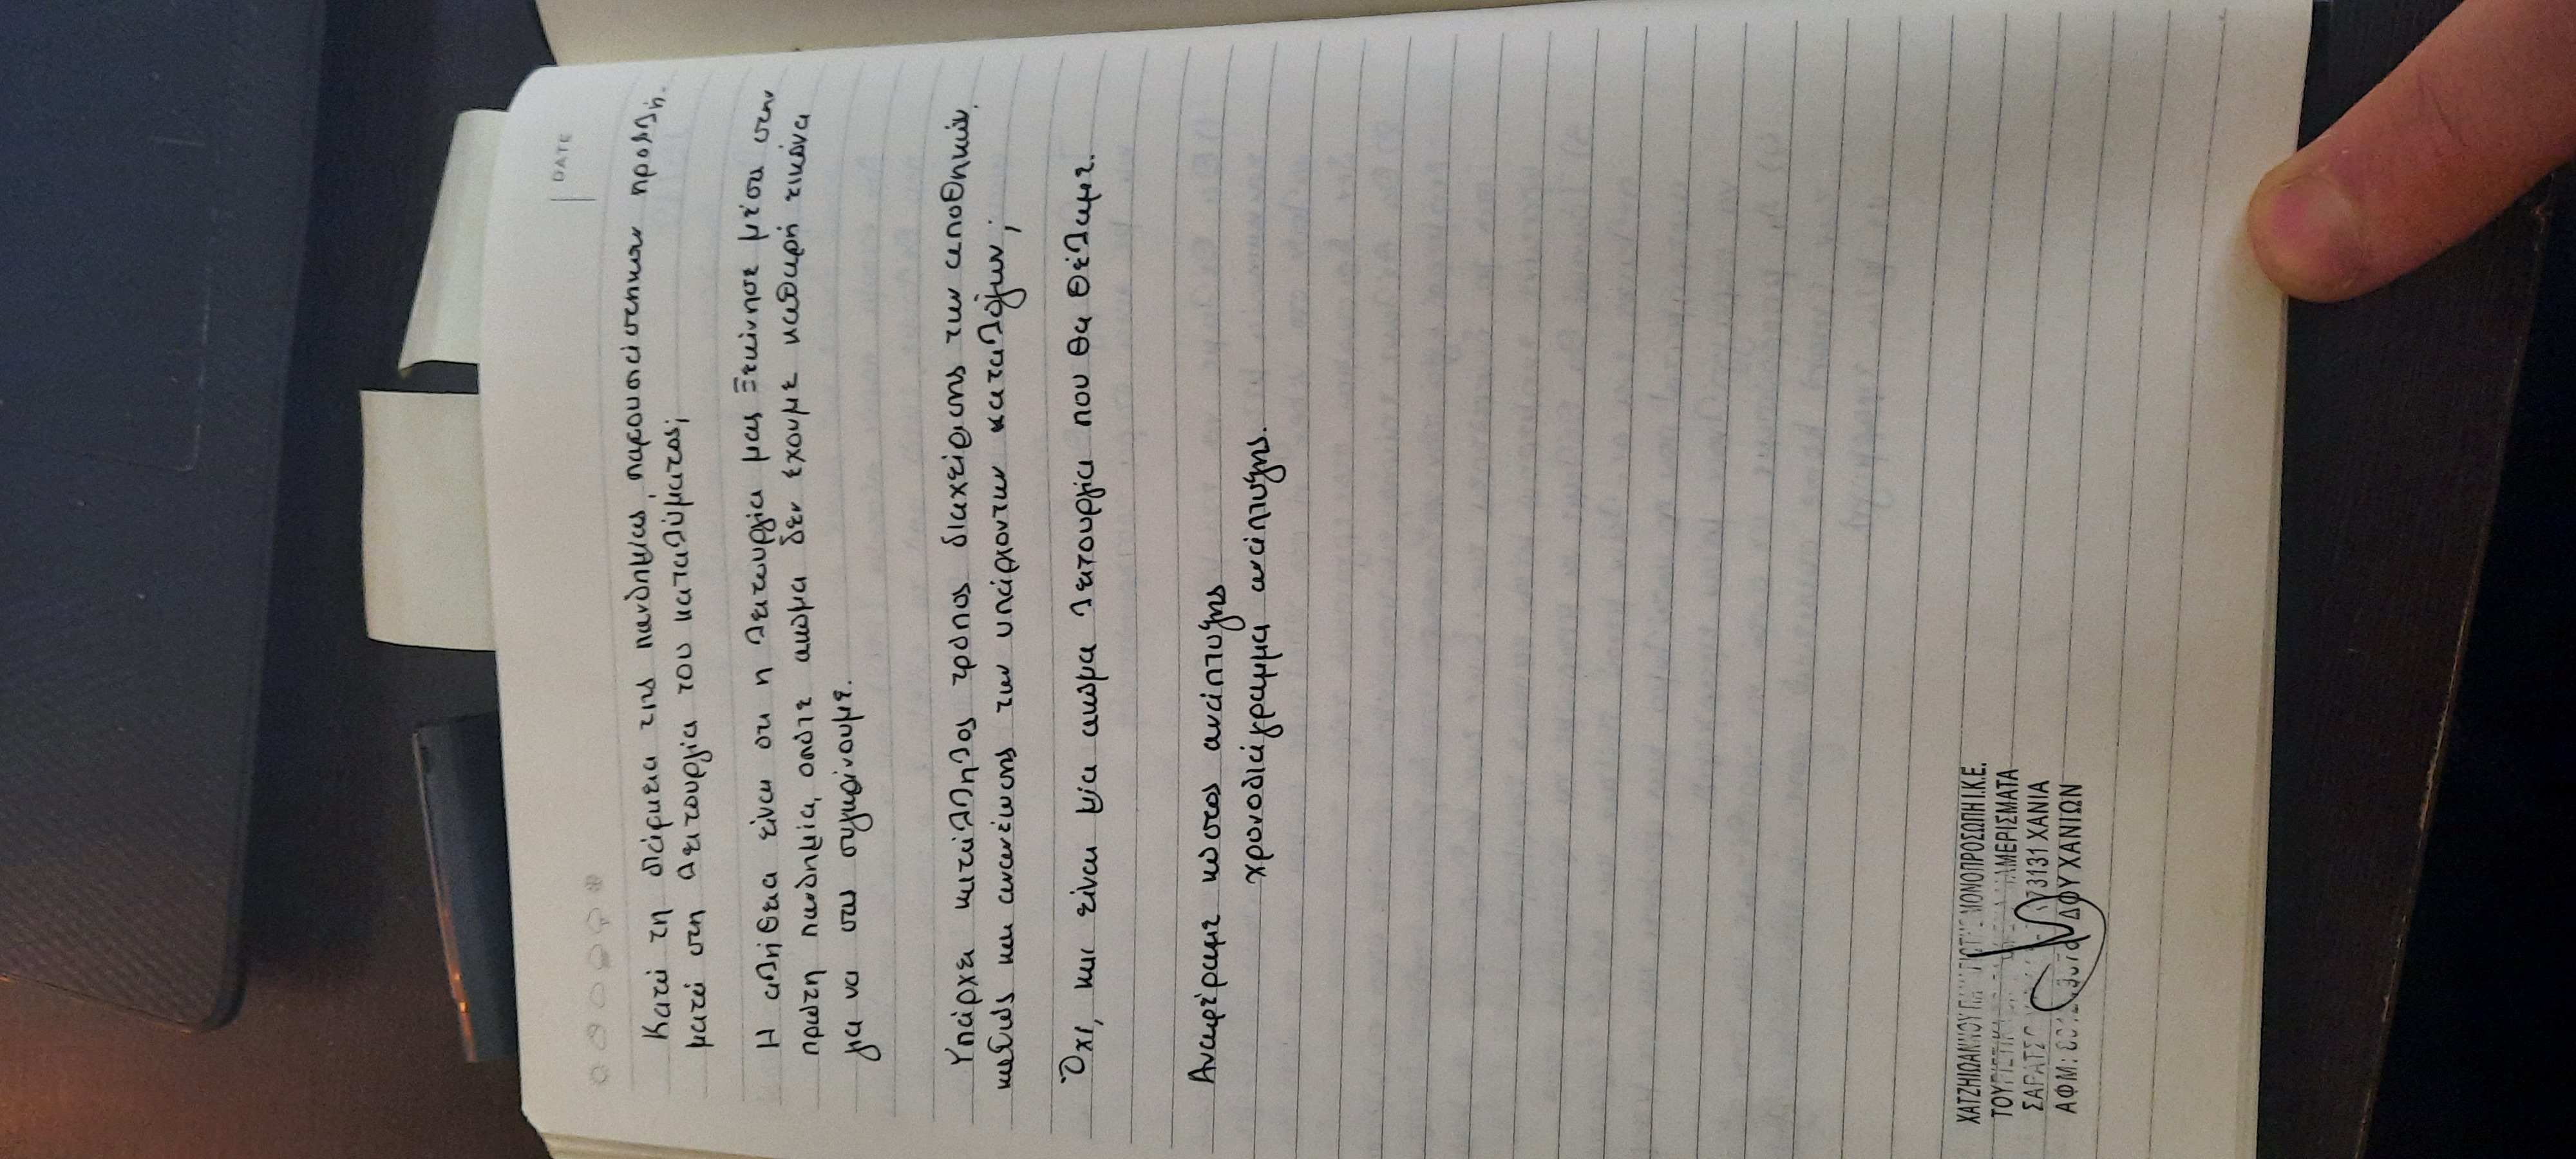
\includegraphics[angle=270, width=0.6\textwidth]{Images/p2}
\end{figure}

\begin{figure}[H]
	\centering
	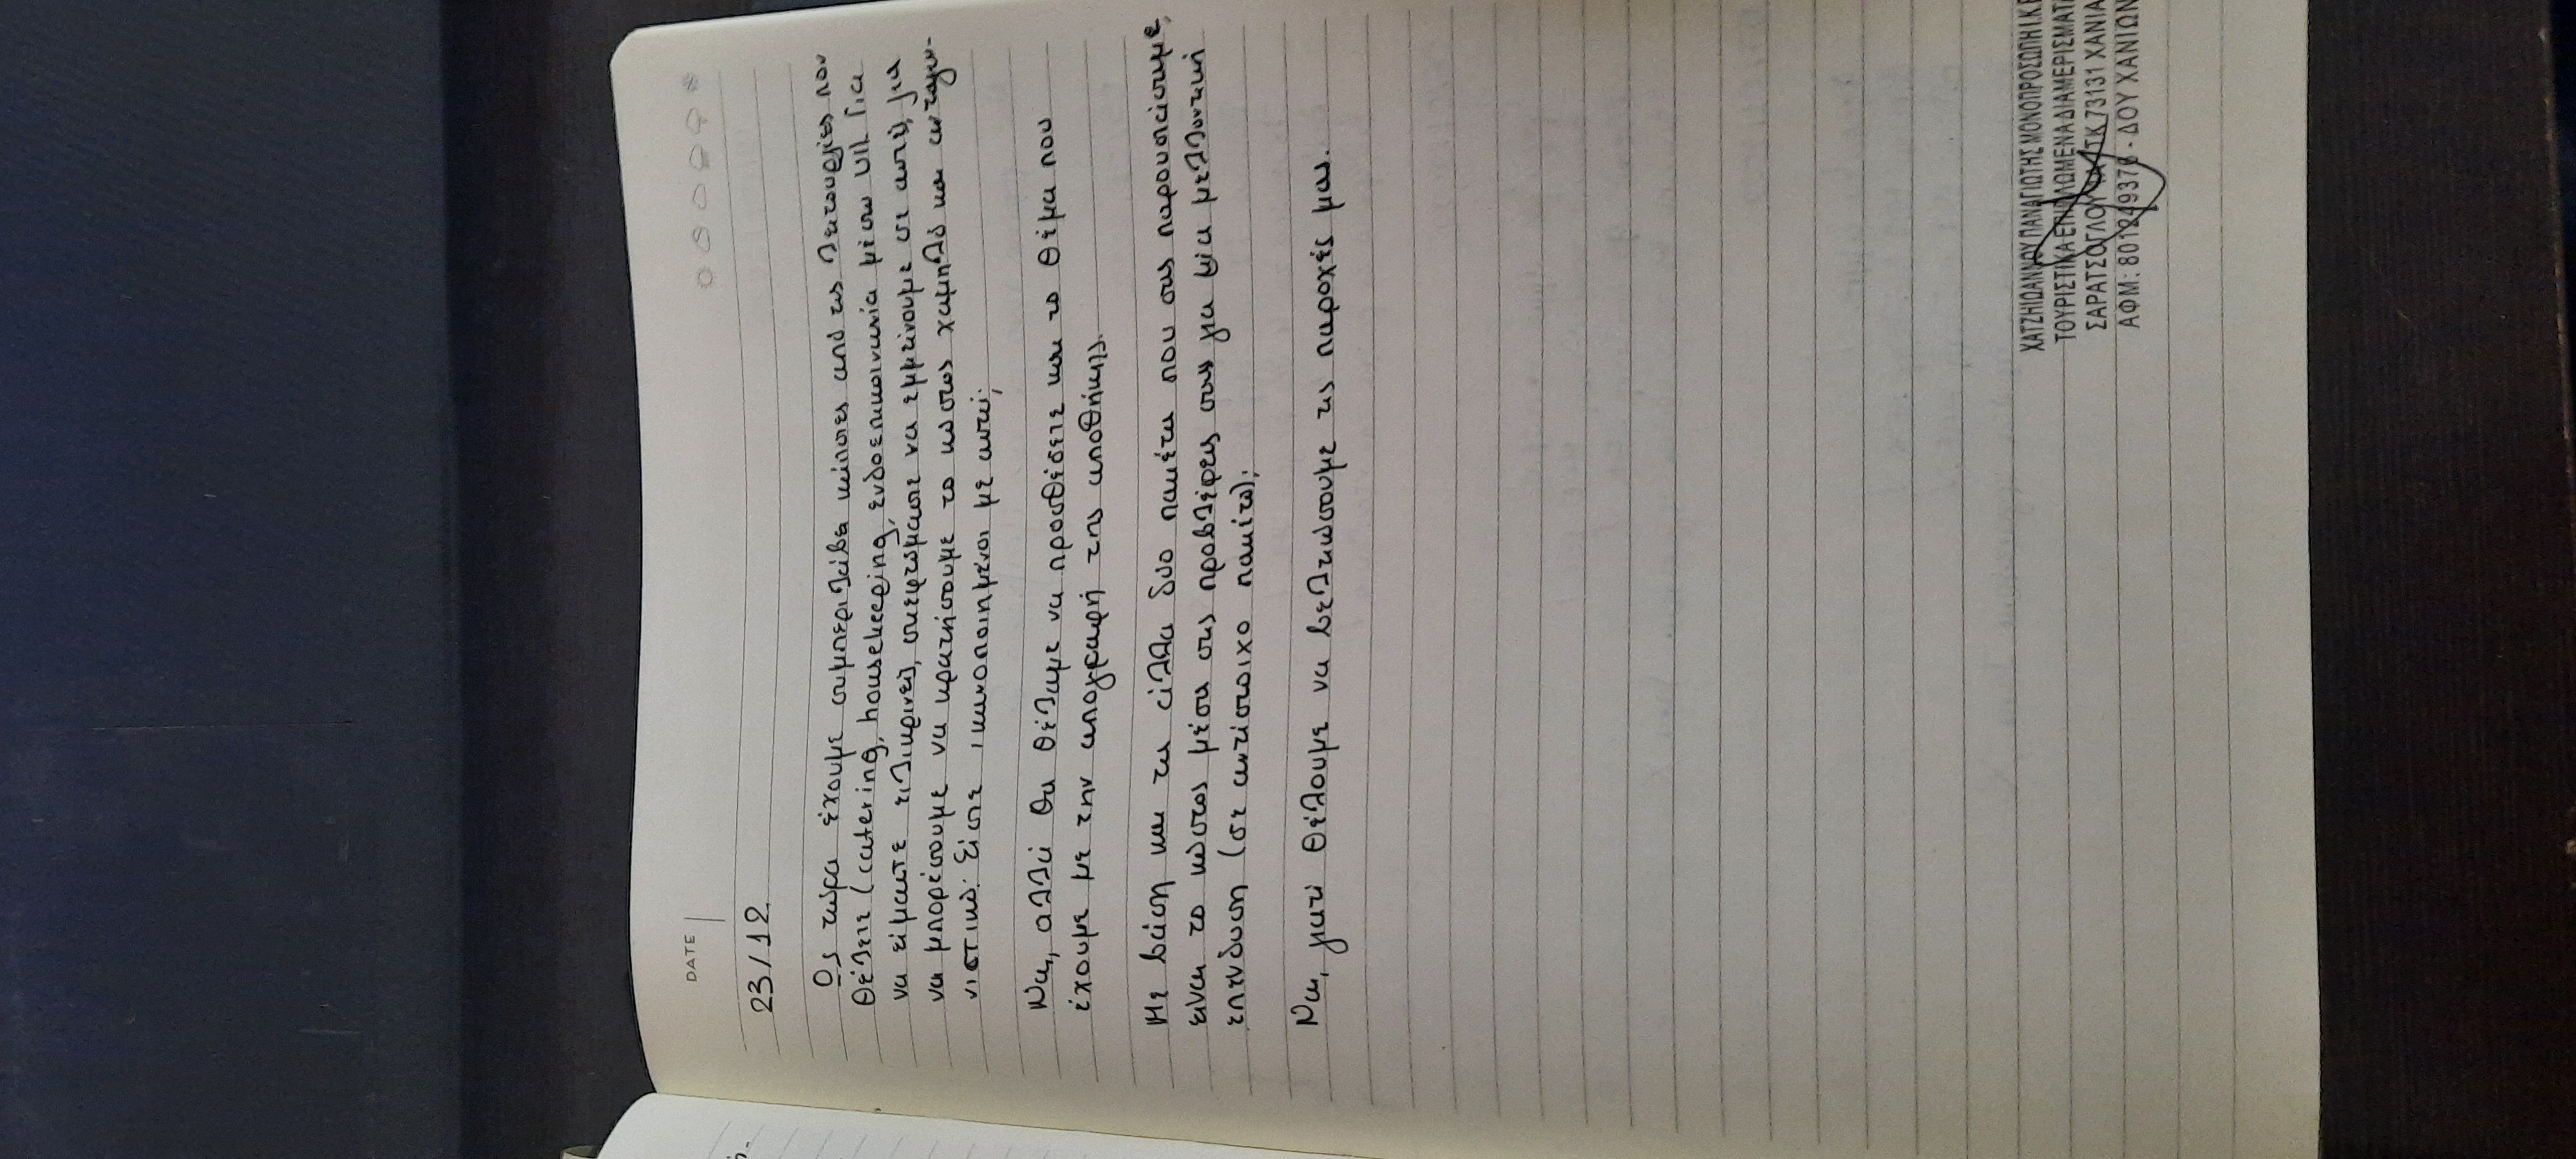
\includegraphics[angle=270, width=0.8\textwidth]{Images/p3}
\end{figure}
